\documentclass[12pt]{article}
\usepackage{blindtext}
\usepackage[en,bordered]{uni-style}
\usepackage{uni-math}

\title{Sheet Vision}
\prof{Professor Khalaj}
\department{Department of Electrical Engineering}
\subtitle{Arad Mahdinejad Kashani, Mehrshad Taji}
\subject{SS Project, Phase 2}
\info{
    \begin{tabular}{lr}
        Arad Mahdinejad Kashani & 400102028\\
        Mehrshad Taji & 400100887
    \end{tabular}
}
\date{\today}
    % \usepackage{xepersian}
    % \settextfont{Yas}
\usepackage{uni-code}
\usepackage{graphicx}
\graphicspath{{pictures/}}
    
\begin{document}
\maketitlepage
\maketitlestart

\section{Find Dr. Khalaj}
The process is fairly simple and straightforward:
\begin{enumerate}
    \item Read the background file
    \item Read the template file
    \item Choose a template matching algorithm (in our case, it was `TM\_CCOEFF')
    \item Choose the best match using `cv.minMaxLoc'
\end{enumerate}

\begin{figure}[h!]
    \centering
    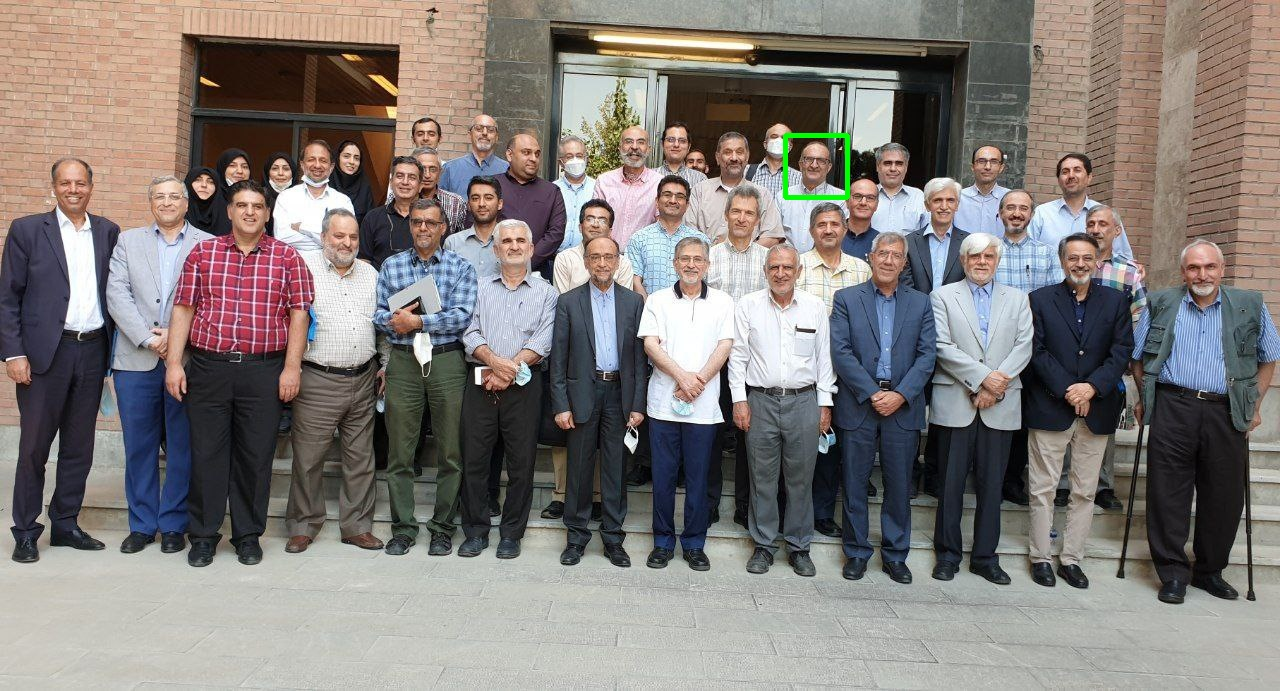
\includegraphics[width=0.7\textwidth]{found khalaj.JPG}
    \caption{Result of Template Matching on the background picture: Dr. Khalaj has been found!}
    \label{fig:1}
\end{figure}
\pagebreak

\section{The MP3 Player}
The raw ipynb file is available on the top folder, as ``mp3player.ipynb''.
\subsection{Overall Algorithm}
The algorithm is simple. We first define a function to create a data structure of 
``how many sample points are in a certain note given a certain tempo and a certain sampling rate $f_s$''. 
This function is available as `getDurations(tempo, fs)'.

This is a simple table for the note durations:
\begin{table}[h!]
\centering
\begin{tabular}{lr} 
    \hline
    \textbf{Note type}& \textbf{Code}\\ 
    \hline
    Whole note& 0\\
    \hline
    Dotted whole note& 1\\
    \hline
    Half note& 2\\
    \hline
    Dotted half note& 3 \\
    \hline
    Quarter note & 4\\
    \hline
    Dotted quarter note & 5\\
    \hline
    etc.
\end{tabular}
\caption{A table for the note durations and their corresponding code.}
\label{table:1}
\end{table}

Then, by editing the ipynb file you provided (``helper.ipynb''), it was possible to integrate
tempo into the functions. Moreover, the ringing was moved so that we could change the ringing
based on the song. I then defined an `attack' value, and knowing how $(t+\alpha)e^{-t}u(t)$ behaves,
by changing the $\alpha$ parameter between 0 and 1, a sense of `attack' was achieved.
This was then multiplied by a corresponding pure sine wave to replicate the notes, giving it an attack and
proper dampening (achieved using the `ring' parameter).

This would go on for $n$ samples, where $n$ is directly in the data structure provided by
`getDurations'. This would then be appended to the previous notes until the end of the song.

\subsection{Convolutional Reverb}
Reverb is a side-effect of sound in an environment, for instance a room, a hall, a stage, etc.
The sound waves will hit the surfaces in the environment and reflect back, with their phases shifted
and a bit of energy loss. This means we can describe overall effect of reverb as:
\begin{equation*}
    y(t) = \sum^{N}_{i=0} \beta_i x(t-\alpha_i)
    \label{eq:1}
\end{equation*}
This is a complex system with too many parameters and is computationally expensive too. \href{https://en.wikipedia.org/wiki/Reverb_effect}
{There are many ways to `fake' a reverb effect}, we chose to use the ``Convolutional Reverb''.
This is a direct result of having equation 1 describe an LTI system; there is an impulse response to the system
and we can use the 1D convolution to calculate the response of this system to any input sound.
Luckily, we were both musicians and one of us had the impulse response pack for many different
rooms and ambiences, some of which are included in the project files for further testing by the reader.

\begin{figure}[h!]
    \centering
    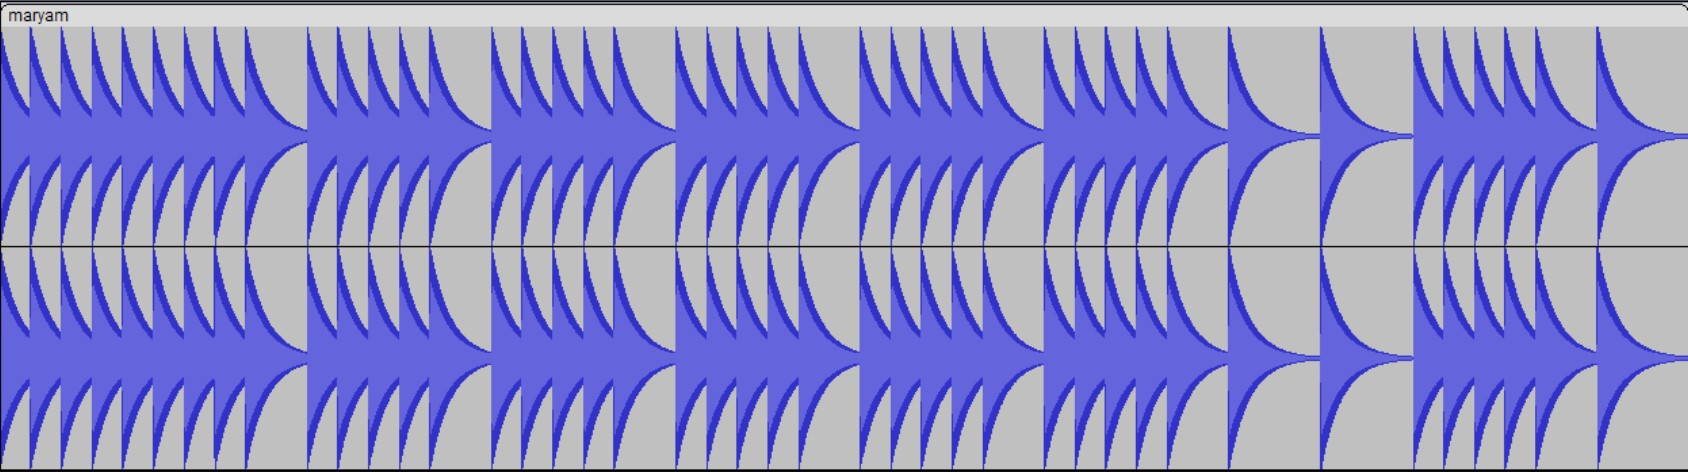
\includegraphics[width=0.5\textwidth]{dry maryam.JPG}
    \caption{``Jane Maryam'' without any effects.}
    \label{dryMaryam}
\end{figure}
\begin{figure}[h!]
    \centering
    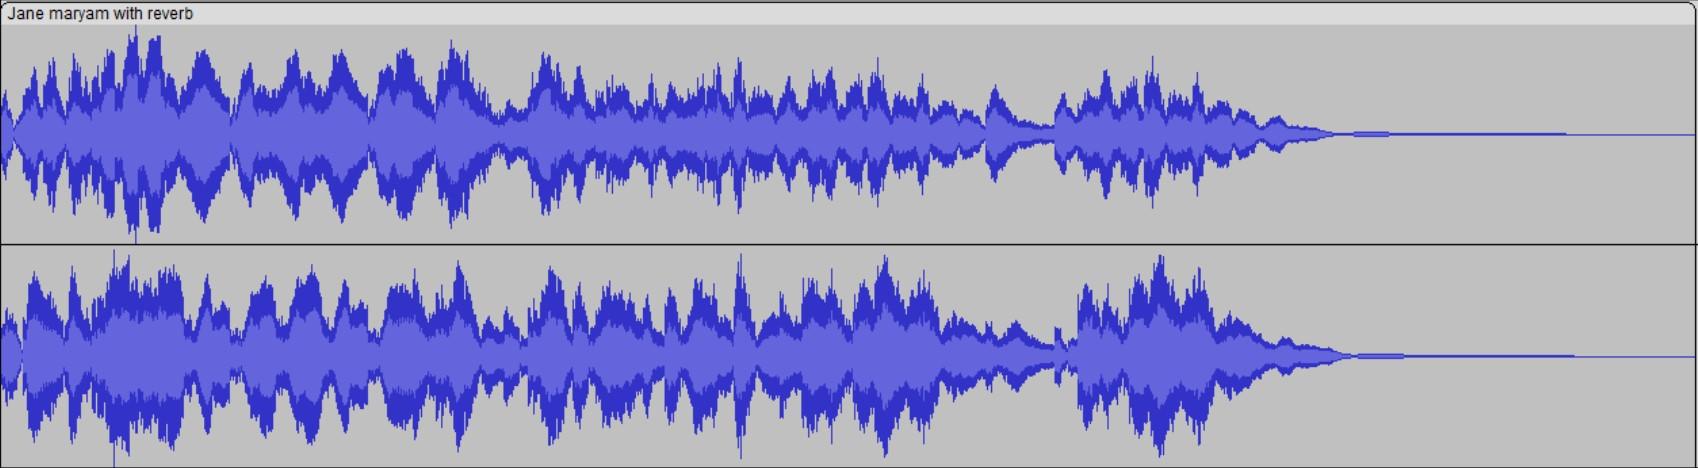
\includegraphics[width=0.5\textwidth]{wet maryam.JPG}
    \caption{``Jane Maryam'' with reverb.}
    \label{wetMaryam}
\end{figure}

Notice how the version with reverb is so much less symmetric, and seems to be much more interesting.
This is a direct result of the room (which was a large hall), making the pure sinusoid sound 
much more `convoluted' and interesting.

\pagebreak

\subsection{Ping-pong delay}
Delays are as simple as it gets: shift a signal to the future by $N$ samples and add it back.
We can easily set $N$ to a distinct number that specifies a legit note duration in our tempo
using `getDurations'. If we have two different delays for the two stereo channels, we have a 
ping-pong delay. This is particularly fun, as you can hear the delays go back and forth in
both ears, especially if one of them is dotted and the other is not.

Denote the dry signal as the original signal, and the wet signal as the delayed signal. Both the dry
and wet signals are being added together.

However, the wet signal seemed too `dry'; so we added a `delay\_effect' function to apply some other effect
to the wet signal before adding it to the dry signal, so that it is less `echo-ey' and more musical.
In the `mp3player.ipynb' file, the effect is a butterworth low-pass filter, with a cutoff frequency of
500Hz.

\subsection{The audio}
Each section's audio file is a .wav file in its own folder, and with its own effects. For instance,
``Jane Maryam'' has a version with reverb and a version without reverb. ``Polyushka Polye'' has a version
with delay and reverb effects both applied, and a dry version too.

The impulse respone for a large hall (used in Convolutional reverb) and demo samples of the C Major scale and ``The Riff''
are available in the `audio/' directory. Other impulse responses are available in the `Impulses/' directory.

\pagebreak

\section{Twinkle Twinkle, Little Star}
We took a screenshot of the .pdf file, and then used that as our image to match its templates.

\subsection{Detecting lines: HoughLines}
We first apply a `cv.Canny' filter, which is basically an edge detector. We then use the
`cv.HoughLines' function to find the location of all the lines in the image. This function
is not very accurate. It returns discontinuous horizontal lines along with vertical lines that
for our uses and purposes, is completely useless and must be removed. 

\begin{enumerate}
    \item At first we remove all the vertical lines. We remove all lines that its starting point and ending points
    share the same $x$ value.
    \item We then sort all the remaining lines by their $y$ coordinates. We take some $y$ margin;
    and count lines closer another line than that value, as duplicates. We then proceed to remove these duplicates.
\end{enumerate}

We then plot the resulting lines.

\begin{figure}[h!]
    \centering
    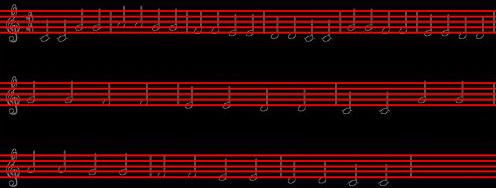
\includegraphics[width=0.7\textwidth]{houghlines.JPG}
    \caption{Result of finding all unique horizontal lines in the image.}
    \label{fig:2}
\end{figure}

\subsection{Note detection}
Now having the line coordinates, we can proceed to find the pitch and duration values of each note.

We first obtain some resources to use as our templates. In this case, it is a stem quarter note.
We then use the `cv.matchTemplate' function to find the notes. We define a threshold, as the output of the
`cv.matchTemplate' function is another image that contains probability values $p$ between 0 and 1 that
determine how `likely' it is for that given pixel to be our template. By using that threshold value,
we can filter out `unlikely' matches and obtain our corresponding notes.

We then filter out the duplicate note detections. We again use the same technique of filtering out note locations
closer than a certain $x$ and $y$ margin.

The results are the top-left corners of the matched template. This is not very useful as we need the location of the center
of the `circular' part of the note. We proceed to add a DC-offset to all the locations to account for this problem, and then
plot the results.

\begin{figure}[h!]
    \centering
    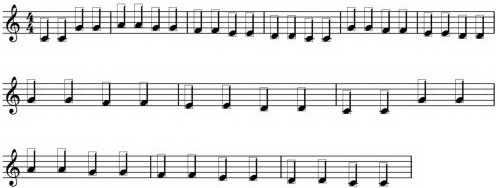
\includegraphics[width=0.7\textwidth]{detected twinkle.JPG}
    \caption{Result of finding notes and removing their duplicates and accounting for offsets.}
    \label{fig:3}
\end{figure}

\pagebreak

\subsection{Compiling the music}
\begin{enumerate}
    \item We first begin by dividing the sheet music into sections. Each section consists of a `line', which is a loose term
    as we are dealing with many lines, but in this case, we mean the collection of all 5 staff lines and their notes. In our
    case, the song ``Twinkle Twinkle, Little Star'' has 3 sections.
    \item We then take each notes' $y$ distance from each line and sort it. There are three possibilites for this:
        \begin{enumerate}
            \item The note is on the line
            \item The note is exactly between two lines
            \item The note is $C_4$ or $D_4$
        \end{enumerate}
    To account for this, we define `onLine\_margin' and `betweenLine\_margin' and `C\_D\_boundary'. Using these parameters, we can
    find which note belongs to what place. Using that, we can determine the pitch values. We then need to account for the durations;
    but in this song all of them are quarter notes. This means that we are done.
\end{enumerate}

We then output the compiled music through the mp3player, and it is available as `TwinkleTwinkle/twinkle.wav'. It contains no effect
and is the raw signal (even without the attack).

\section{Ave Maria}
The process is not that different from the process used in ``Twinkle Twinkle, Little Star'', the only difference is that we now have
different duration values. Using the same techniques, we find the locations, and using another resource for the half note, we append the
duration value to the location value; such that the data structure looks something like [$x$, $y$, duration].
In the compilation stage, we use the duration value and pass it to mp3player, where it will be processed there.

The ending result is available as `AveMaria/avemaria.wav', without any effects.

\begin{figure}[h!]
    \centering
    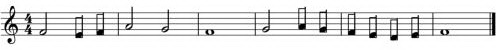
\includegraphics[width=0.7\textwidth]{detected ave.JPG}
    \caption{Result of adding duration handling.}
    \label{fig:4}
\end{figure}

\section{Polyushka Polye}
The challenge for ``Polyushka Polye'' is that we have pitch accidentals. We again append another property to each note.
This pitch shift property will determine how many semitones we should offset from the origin. 0 is the original pitch,
and this is why all notes will be initialized to 0 pitch shift. We then proceed to detect all sharps and flats \underline{in their own
sections}, and then find the note with the closest $x$-value to the accidental. We then change the pitch shift property accordingly.


The dry version is available as `Polye/polye.wav', and a version with delay and reverb is available
as `Polye/Polye with reverb and delay.wav'.
\begin{figure}[h!]
    \centering
    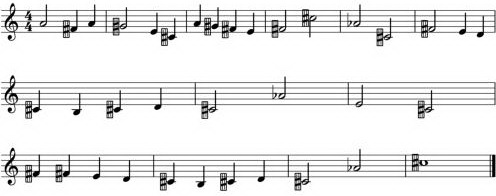
\includegraphics[width=0.7\textwidth]{detected polye.jpg}
    \caption{Results of detecting the accidentals}
    \label{fig:5}
\end{figure}

\section{Jane Maryam}
The process for ``Jane Maryam'' is very similar to the process for ``Polyushka Polye'', as pitch accidentals are very similar to dotted notes.
We apply the same logic, and as the duration list for notes in mp3player was arranged for this exact reason, the matched note for each dot
will have its durations value added by 1.

The dry output is available as `JaneMaryam/maryam.wav' and a version with reverb is available
as `JaneMaryam/Jane maryam with reverb.wav'.

\makeendpage
\end{document}